\section{Transforming Coordinate Systems}
\label{key:data:cs}
Usually, \PGFPlots\ works with cartesian coordinates. However, one may want to provide coordinates in a different coordinate system.

In this case, the |data cs| key can be used to identify the input coordinate system:

\begin{pgfplotskey}{data cs=\mchoice{cart,polar,polarrad} (initially cart)}
	Defines the coordinate system (`cs') of the input coordinates. \PGFPlots\ will apply transformations if the argument does not match the expected coordinate system.

	Use |data cs| if your input has a different coordinate system than the axis. More precisely,
	every axis type has its own coordinate system. For example, a normal |axis| has the |cart| coordinate system, whereas a |polaraxis| has a |polar| coordinate system. The use of |data cs| with a different argument than the default of your axis instructs \PGFPlots\ to apply transformations.
	
	At the time of this writing, \PGFPlots\ supports the following values for |data cs|:

	The |data cs=|\declareandlabel{cart} denotes the cartesian coordinate system. It is the coordinate system of the usual |axis| (or its logarithmic variants). It can have three components, $x$, $y$, and $z$. Specifying it is only necessary if you have a non-cartesian axis:
% \usepgfplotslibrary{polar}
\begin{codeexample}[]
% requires \usepgfplotslibrary{polar}
\begin{tikzpicture}
	\begin{polaraxis}
	\addplot coordinates {(90,1) (180,1)};
	\addplot+[data cs=cart] 
		coordinates {(1,0) (0.5,0.5)};
	\end{polaraxis}
\end{tikzpicture}
\end{codeexample}

	The |data cs=|\declareandlabel{polar} is the (two--dimensional) coordinate system with (angle, radius), i.e.\ the first component ``$x$'' is the angle and the second component ``$y$'' is the radius. The angle is a number in the periodic range $[0,360)$; the radius is any number. If a |polar| coordinate has a $z$ component, it is taken as-is (the transformations ignore it).
\begin{codeexample}[]
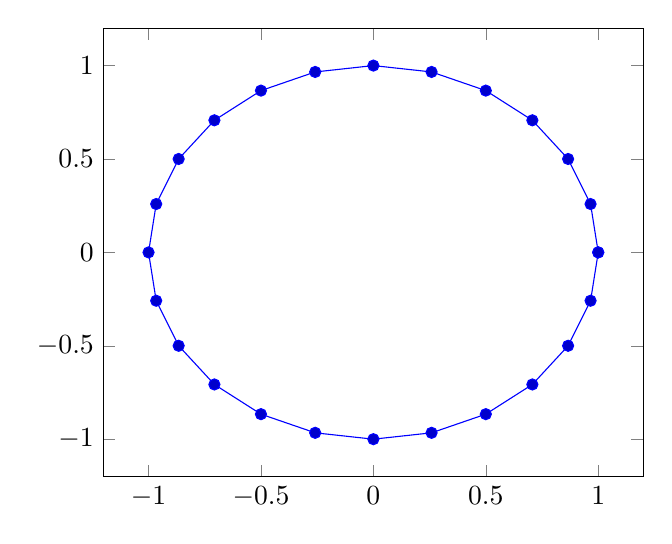
\begin{tikzpicture}
	\begin{axis}
	\addplot+[data cs=polar,domain=0:360] (\x,1);
	\end{axis}
\end{tikzpicture}
\end{codeexample}

	The |data cs|=\declareandlabel{polarrad} is similar to |polar|, but it expects the angle in radians, i.e.\ in the periodic range $[0,2\pi)$.
\begin{codeexample}[]
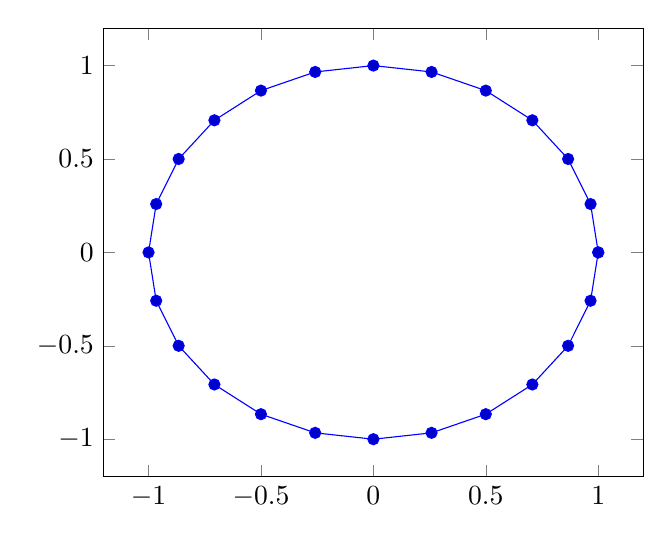
\begin{tikzpicture}
	\begin{axis}
	\addplot+[data cs=polarrad,domain=0:2*pi] (\x,1);
	\end{axis}
\end{tikzpicture}
\end{codeexample}

	Note that the math function |deg(|\meta{rad}|)| transforms \meta{rad} into degrees and |rad(|\meta{degree}|)| transforms \meta{degree} into radians. Consequently, |polar| and |polarrad| are more-or-less equivalent for plot expression.

\begin{codeexample}[]
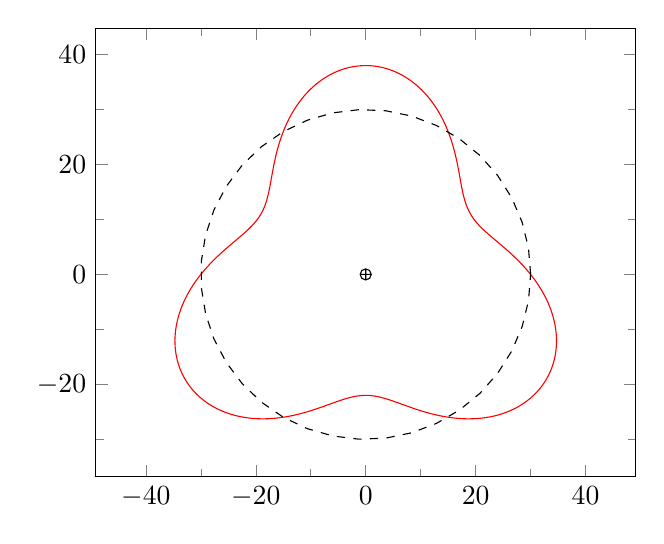
\begin{tikzpicture}
 \begin{axis}[
 	axis equal,
	minor tick num=1,
]
\def\FREQUENCY{3}
\addplot[red,domain=0:360,samples=200,
	smooth,data cs=polar] 
	(x,{30-8*sin(\FREQUENCY*x)});

\addplot[samples=40,domain=0:2*pi,dashed,
	data cs=polar] (deg(x),30);

\addplot[mark=oplus,only marks] coordinates {(0,0)};
 \end{axis}
\end{tikzpicture}
\end{codeexample}


	At the point of this writing, the |data cs| method will work for most plot handlers. But for complicated plot handlers, further logic may be needed which is not yet available (for example, the |quiver| plot handler might not be able to convert its direction vectors correctly)\footnote{In case you run into problems, consider writing a bug report or ask others in \TeX\ online discussion forums.}.
\end{pgfplotskey}

\begin{command}{\pgfplotsaxistransformcs\marg{fromname}\marg{toname}}
	Expects the current point in a set of keys, provided in the coordinate system \meta{fromname} and replaces them by the same coordinates represented in \meta{toname}.

	On input, the coordinates are stored in |/data point/x|, |/data point/y|, and |/data point/z| (the latter may be empty). The macro will test if there is a declared coordinate transformation from \meta{fromname} to \meta{toname} and invoke it. If there is none, it will attempt to convert to |cart| first and then from |cart| to \meta{toname}. If that does not exist either, the operation fails.
\end{command}

\begin{command}{\pgfplotsdefinecstransform\marg{fromname}\marg{toname}\marg{code}}
	Defines a new coordinate system transformation. The \meta{code} is expected to get input and write output as described for |\pgfplotsaxistransformcs|.

	Implementing a new coordinate system immediately raises the question in which math mode the operations shall be applied. \PGFPlots\ supports different so--called ``coordinate math systems'' for generic operations, and for each individual coordinate as well. These coordinate math systems can either use basic \PGF\ math arithmetics, the |fpu|, or perhaps there will come a Lua\TeX\ library.

	The documentation of this system is beyond the scope of this manual\footnote{Which is quite comprehensive even without API documentation, as you will certainly agree...}. Please consider reading the source-code comments and the source of existing transformations if you intend to write own transformations.
\end{command}

\subsection{Interaction of Transformations}
\label{sec:transformation:interaction}

There are a couple of coordinate mappings in \PGFPlots. For each encountered coordinate in a coordinate stream (|\addplot|), it applies the following steps:
	\begin{enumerate}
		\item Remember the ``raw'' coordinates in math constants |rawx|, |rawy|, |rawz|,
			\index{rawx}\index{rawy}\index{rawz}%
		\item Apply |pre filter|,\index{pre filter}
		\item Apply |x coord trafo|, logarithm if necessary, and |x filter| (in this order),%
			\index{x coord trafo}%
		\item Apply |y coord trafo|, logarithm if necessary, and |y filter|,
			\index{y coord trafo}%
		\item Apply |z coord trafo|, logarithm if necessary, and |z filter|,
			\index{z coord trafo}%
		\item Apply |filter point|,
			\index{filter point}%
		\item Transfrom from |data cs| to the coordinate system of |axis type|,
			\index{data cs}%
		\item Handle coordinate stacking (|stack plots=x| and/or |stack plots=y|).
			\index{stack plots}%
	\end{enumerate}
Here, |pre filter| takes no arguments; it simply prepares the following filters. Consequently, the first item which actually accepts the input argument is |x coord trafo|. This method is part of the parsing; it accepts the ``raw'' coordinate which may be in symbolic form. The output of |x coord trafo| and its variants is a number. This number can be filtered or transformed by means of |x filter| and its variants. Note that |x filter| simply takes one argument: the result of |x coord trafo|. 

The intented meaning of |x coord trafo| is to define how the ``raw'' string form as provided by the user makes its way into \PGFPlots. It is also the only transformation which has an inverse, the key |x coord inv trafo|. The inverse can be used to transform back from internal numeric form to some string for the end user. The key |x coord trafo| can only be defined as option to an axis, i.e.\ it it cannot be provided to |\addplot|.

The meaning of |x filter| and its variants is to transform numbers or to conditionally throw away numbers (and thus the entire coordinate). Each |\addplot| can receive its own (set of) filters.

The key |filter point| accepts \emph{all} arguments (more precisely: the result of the preceding steps). It can rely on $x$, $y$, and $z$, and it can change any of them. The way it accepts the coordinates is by means of keys |/data point/x|\index{/data point/x} and its variants for $y$ and $z$. In principle, |filter point| is the most general filter. However, you can define both |x filter| and |filter point|, and both will be applied. Each |\addplot| can receive its own |filter point|.

The implementation for the key |data cs| is similar to |filter point| in that it accepts the result of all previous mapping steps. However, it maps from a well--defined input coordinate system to some well--defined internal coordinate system (which is inherent to the axis). Each |\addplot| can receive its own |data cs|.

Finally, |stack plots| takes measures to add/subtract the results. Stacking of plots is a property of the axis; it is not intented to be provided as argument to |\addplot|\footnote{Also it appears to do something which is not entirely useless.}.

